\chapter{Related Work}
\lettrine[lines=4, loversize=-0.1, lraise=0.1]{I}{n the following} chapter we present previous work done in the area, both in research and in product development.The chapter is divided into the two topics Speech Recognition an Natural Language Processing and Requirement Management. 

\section{Speech Recognition}
In recent years, personal assistants using speech recognition have been released, such as Siri \citep{sirirelease} and Google Now~\citep{googlenowrelease}. These applications interprets input from a users speech, and dependent on the interpreted input, performs an action and presents the outcome of the action. These actions could be entering a string in a search engine and present the result, or setting an alarm at a spoken time. A list of available voice actions in Android can be seen in Figure~\ref{fig:voiceactions}.

\begin{figure}[h]
\centering
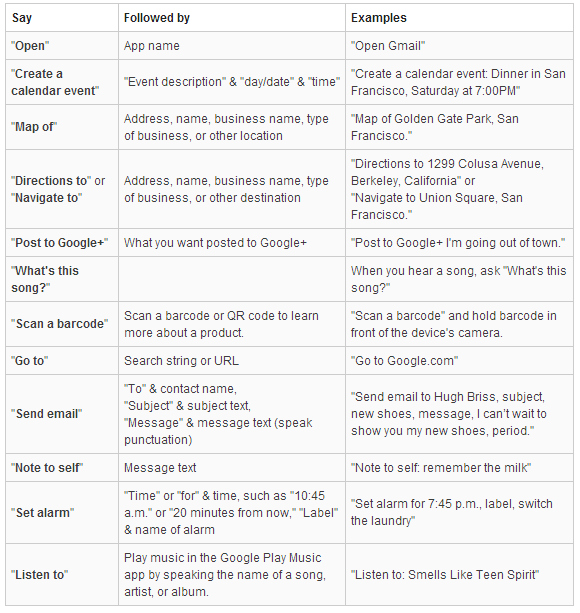
\includegraphics[width = 400pt, keepaspectratio = true]{fig/voiceactions.png}
\caption{Examples of different voice actions in Android \citep{voiceactions}}
\label{fig:voiceactions}
\end{figure}
\FloatBarrier

Moreover, Nuance has developed a Software called Dragon Naturally Speaking which allows for a user to use their voice as the input channel to a computer. Dragon Naturally Speaking allows for the user to create and edit documents and emails, as well as launching applications or controlling a computer mouse, all through  spoken commands \citep{nuancedragon}.
\section{Natural Language Processing}
\label{sec:natlangprocsess}
The following section will present former research and techniques used in Natural Language Processing. The section presents methods for processing natural language text to produce unambiguous data, and discusses string edit distance functions as a method to find similarities or dissimilarities between strings.

\subsection{Information Extraction and Information Retrieval}
In natural language processing, Information Extraction (IE), the process of taking unseen text as input and producing fixed-format, unambiguous data as output, has been researched and implemented in different ways over the years. In 2000, \citet{cunningham2000} presented five different types of IE: 

\begin{itemize}
  \item \textbf{Named Entity recognition (NE):} Which finds entities in texts, such as places, names, organizations etc.
  \item \textbf{Co-reference resolution (CO):} Which identifies the \emph{identity} relationships between the found entities, i.e.\ if two different words refers to the same person (Ms. Smith and she).
  \item \textbf{Template Element construction (TE):} Who adds descriptive information to the found entities using the the relationships found in CO.
  \item \textbf{Template Relation construction (TR):} Which extracts the relationships between the Template Elements, i.e.\ the relationship between entities (Ms.Smith studies at Chalmers).
  \item \textbf{Scenario Template production: (ST)} Who take the results found in TE and TR and matches them into event scenarios
\end{itemize}

Another process in NLP is Information Retrieval (IR) which is the process of finding relevant text and present them to users (typical use case would be an Internet search engine). 

\subsection{String Edit Distance Functions}
\label{subsec:sedf}
Speech recognition, as stated, has over the recent years become more efficient and accurate, but there are still limitations.
One way to mitigate these limitations, which was deployed in this research, is to use natural language processing and string distance functions, e.g. the Levenshtein or Hamming distance algorithms~\citep{levenshtein,hamming}. 
These algorithms calculates similarities or dissimilarities between string by measuring how many operations (add, modify, delete) that are needed to transform one string to another.

\section{Requirement management and NLP}
\citet{joshi2012} showed that natural language can be integrated into the creation of software artifacts. A tool which extracts UML-diagrams from natural language was developed with a precision and recall rate of 85\%. The method used was to apply already existing natural language parsers and then apply algorithms to filter and correct the words, remove suffixes and affixes, as well as identifying classes, attributes and relationships.

\citet{gervasi2002} conducted a case study with the aim to validate natural language requirements. The validation was made possible by implementing the process of validation into two steps, \emph{set-up} and a \emph{production phase}. 

In the \emph{set-up}, the rules of the domain was defined. Rules of style, structure and language of the requirement document, as well as which properties that were desirable to check, and finally defined models who the selected properties could be checked against. In the second phase, the \emph{production phase}, the document with the natural language was pre-processed and then parsed with regards to the defined properties. This parsing process provided a validation of the syntactic language in the document \citep{gervasi2002}.

%In 2000, Berglund wrote an article titled 'Writing for Adaptable Documentation'. He talks about adaptable documentation and change mechanics. In the conclusion he presented that 
%\begin{quotation}"The documentation must contain information about how to adapt. Information designers therefore need tools that encapsulate change semantics and provide clear concepts for adaptivity" \citep{berglund2000}
%\end{quotation}